\documentclass{tongjithesis}
\usepackage{tongjithesis}

%%%%%%%%%%%%%%%%%%%%%%%%%%%%%%%%%%%
% 若你想要用句点(.)替换句号(。)
% 可以打开下面的注释
%%%%%%%%%%%%%%%%%%%%%%%%%%%%%%%%%%%
% \catcode`\。=\active
% \newcommand{。}{\ifmmode\text{.}\else .\fi}
%%%%%%%%%%%%%%%%%%%%%%%%%%%%%%%%%%%

%%%%%%%%%%%%%%%%%%%%%%%%%%%%%%%%%%%
% 默认使用 Adobe Times Roman
% 如果你想使用 Times New Roman
% 可以打开下面的注释来覆盖 mathptmx
%%%%%%%%%%%%%%%%%%%%%%%%%%%%%%%%%%%
%\usepackage{fontspec}
%\setmainfont{Times New Roman}
%%%%%%%%%%%%%%%%%%%%%%%%%%%%%%%%%%%
\begin{document}

\school{电子与信息工程学院}
\major{计算机科学与技术}
\student{1953080}{田宇}
\thesistitle{基于可信执行环境的安全高效微服务计算平台}{}
\thesistitleeng{A Secure and Efficient Microservice Computing Platform Based on Trusted Execution Environment}{}
\thesisadvisor{崔鹤鸣、邓蓉}
\thesisdate{2023}{06}{06}

\MakeCover


\pagestyle{firststyle}
\MakeAbstract{
    微服务架构将单一服务程序划分为一组独立的、小型的微服务,已经成为了一种日渐流行的面向服务架构形式,并得到了广泛的应用。但是微服务架构也带来了一些新的挑战:使用公有云的微服务需要信任公有云,以保证其不会窃取隐私数据,限制了公有云微服务的使用场景;微服务节点间的频繁通信带来了极大的网络攻击面,并带来了更大的总通信延迟。

    为了保障运行环境的安全性和通信的安全和高效性,我们针对微服务安全计算场景的特点,设计实现了一个基于可信执行环境的安全高效微服务计算平台,包含一个细粒度、模块化的运行时系统以及一个安全高效的通信协议。我们的运行时具有较小的TCB,并通过借助Intel SGX提供的保护,可以避免特权态攻击;我们的通信安全协议结合了TLS和SGX远程验证的特点,能够防御中间人攻击和重放攻击,确保通信节点的合法性,并能够实现更小的通信延迟。

    为了验证平台的性能,我们还设计实现了一个图像处理微服务示例应用。该应用使用Rust语言实现,用以保障程序本身的安全性;该应用使用gRPC进行通信并使用Token交换的授权管理方式,能够实现高效通信和细粒度的授权管理。我们在云服务器上进行了测试,结果表明,我们的平台达到了安全高效的微服务计算的设计目标。
}{微服务,可信执行环境,Intel SGX,运行时,安全通信协议,Rust语言,安全性}

\MakeAbstractEng{
    Microservices architecture has become a popular form of service-oriented architecture that involves dividing a single service program into a group of independent, small microservices. However, this architecture also brings new challenges. Using microservices on public clouds requires trust in the cloud provider to ensure they do not steal private data, limiting the use cases of public cloud microservices. Frequent communication between microservice nodes also increases the attack surface and total communication latency.

    To ensure the security and efficiency of the runtime environment and communication, we designed and implemented a secure and efficient microservices computing platform based on trusted execution environment, which includes a fine-grained, modular runtime system and a secure and efficient communication protocol. Our runtime has a small TCB and can prevent privileged mode attacks by leveraging the protection provided by Intel SGX. Our secure communication protocol combines the features of TLS and SGX remote attestation, which can defend against man-in-the-middle and replay attacks, ensure the legitimacy of other nodes, and achieve lower communication latency.

    We also designed and implemented a sample image-processing microservice application to verify the platform's performance. The application is implemented in Rust to ensure the program's security. It uses gRPC for communication and Token exchange method for authorization, enabling efficient communication and fine-grained authorization management. We tested the platform on a cloud server, and the results show that our platform achieves the design goal of secure and efficient microservices computing.
}{Microservice, TEE, Intel SGX, Runtime, Secure Communication Protocol, Rust, Security}


\clearpage
\tableofcontents   %放置目录
\clearpage

\pagestyle{mainstyle}
\section{引\ 言}\label{sec:introduction}

随着面向服务架构(SOA)的发展,微服务~\cite{lewis2014microservices}已经成为了一种日渐流行的架构风格,并得到了工业界的广泛采用(例如Netflix的视频点播服务~\cite{msnetflix}和Google的云存储服务~\cite{msgoogle}等)。与传统的单一服务(monolithic service)模式不同,微服务架构将一个庞大的服务拆分为多个独立的、简单的、解耦合的微服务,通过网络进行通信,每个微服务都可以独立部署、升级、扩展,因此可以突破传统软件架构的限制,大大提升软件开发的灵活性和效率。

% 微服务架构的典型应用场景包括:Netflix的视频点播服务~\cite{}、Amazon的电子商务服务~\cite{}、Uber的叫车服务~\cite{}等等。

但是,在提供了开发、部署等方面的灵活性和便利性的同时,微服务架构也带来了一些新的挑战,并引入了许多新的攻击面。

首先是运行环境的安全问题。微服务通常部署在公有云PaaS上,PaaS(平台即服务)\cite{mell2011nist}是一种云计算模型,提供了可用于开发、运行和管理应用程序的完整的云平台(包括硬件、软件和基础设施),并提供了自动化扩展的能力。然而,使用PaaS的微服务需要信任公有云,以保证其不会窃取用户的私密信息;如果公有云平台是恶意的或者被恶意攻击者劫持,很容易威胁到其上运行的微服务的安全性。因此,公有云限制了微服务的应用场景(如人脸数据处理等)。

另外,微服务节点间的通信也面临新的挑战。由于分布式、解耦合的特点,微服务节点之间需要频繁的通信,这在单一服务的基础上额外引入了通信攻击面,对微服务架构的通信安全和节点认证等方面提出了挑战。例如,微服务节点之间的通信可能会被窃听、篡改,从而导致数据泄露、数据篡改等问题;恶意的或被劫持的节点可能会骗取正常节点的信任,从而窃取正常节点的机密信息,造成隐私泄露。同时,大量微服务节点的多级通信关系也对通信的效率提出了挑战,研究表明,传统的单一服务只需要满足百毫秒级别的延迟要求即可对用户提供高质量的服务,而微服务场景下节点间的通信需要满足亚毫秒(sub-ms)的要求,才能在总体延迟上达到和单一服务相近的效果~\cite{sriraman2018mutune}。

因此,为了保障安全计算场景下微服务的安全性(security),我们需要从运行时环境和网络通信两方面入手,二者缺一不可;例如如果只保护了运行时数据安全,但是网络通信遭到了攻击,仍然会威胁整个服务平台的机密性和完整性,反之亦然。

为了保障微服务运行时的安全,我们可以借助可信执行环境(TEE)~\cite{sabt2015trusted}的力量。可信执行环境是一种硬件级别的安全容器,通过CPU创建安全的飞地(Enclave),可以对运行在其内部的代码、数据提供机密性、完整性的支持,从而保护微服务应用的安全。因为可信执行环境结合了密码学原理和硬件级别的保护,可以在不信任公有云系统的情况下保护数据的机密性和完整性,即使云上系统是恶意的或被劫持,也能保护飞地中的数据。另外,因为有些TEE的内存不能过大,且为了减少攻击面,需要控制可信信任基(TCB)的大小,这与微服务独立而微小的特点是天然符合的。

目前主流的公有云大多是Intel架构的,因此我们选择使用Intel SGX~\cite{costan2016intel}来提供保护;但是由于SGX主要提供的是硬件级别的隔离,只包含基本的库函数而不能提供POSIX接口,不能直接移植现有的程序,因此我们需要在SGX的基础上针对微服务的特点设计合适的运行时系统,以支持微服务的运行。

目前SGX上的运行环境主要有两种设计思路。第一种是在SGX中运行一个小型的操作系统,比如Microkernel(例如Keystone~\cite{lee2020keystone}的运行时)或LibOS(例如Graphene-SGX~\cite{tsai2017graphene}等),这样可以在无改动或极少改动的情况下将现有程序运行在SGX中;但是这样会包含较多的代码,具有较大的TCB,可能存在较多漏洞和较大的攻击面。第二种思路是针对特定编程语言编写SGX内的运行时库(例如Rust-SGX~\cite{wang2019towards}、GoTEE~\cite{ghosn2019secured}等),这样可以达到很小的TCB;但是这种方式只能针对特定的编程语言,且不能实现所有的系统功能。在本课题中,根据微服务应用的特点,我们设计了一种将二者结合的细粒度、模块化的运行时实现方式,能够在较小TCB的情况下为应用提供SGX的保护。

为了保障微服务节点通信的安全,我们需要安全高效的远程验证协议和通信协议。在微服务场景下的网络通信需要提供4层保障,分别是用户端和服务端的验证、微服务节点间互相验证对方的身份和合法性、微服务节点间通信的机密性和完整性保障、依赖节点间授权合法性的验证。其中,第一种情况是SOA架构固有的问题而不是微服务架构新引入的问题,关于这个问题的解决已有成熟的方案(例如OAuth2~\cite{oauth2spec}等),因此本次研究可以不考虑;第二种情况要确认对方身份合法并且运行在一个符合规范的SGX实体中,这一点可以通过Intel的SGX远程验证~\cite{intel-sgx-ra}进行;第三种情况主要面对的是网络上的攻击,例如中间人攻击(MITM)和重放攻击(Replay Attack)等,也已经有了较成熟的解决方案(例如TLS协议~\cite{8446});最后一种情况是应用开发者的职责,需要进行细粒度的授权划分,可以使用基于Token交换的授权方案~\cite{rfc8693}。本次设计针对微服务安全计算的场景,将TLS、SGX远程验证和Token交换结合起来,设计了一种新的安全高效的安全通信协议。
% 在通信性能方面,我们参考了几种常见远程过程调用(RPC)框架(例如gRPC~\cite{}、Thrift~\cite{}等)的性能,以及RPC与HTTP协议的性能的对比~\cite{},选择使用高效的gRPC来进行微服务节点间的通信。

另外,为了减小TCB,我们难以使用运行时内存占用较大的语言(例如脚本语言)编写微服务节点,而需要使用系统编程语言(例如C~\cite{kernighan1988c}、C++~\cite{stroustrup2013cpp}、Rust~\cite{rust-lang}等)。由于需要高安全性保障的微服务节点通常是处理敏感数据或涉及到敏感业务的,在所有节点中占据比重较低,因此这种对于编程语言的限制是合理的。然而,尽管可以通过非技术手段保障节点不是恶意的,但是我们不能保证使用系统语言编程的微服务节点不会出现漏洞(例如缓冲区溢出、悬垂指针等),这些问题会严重危害系统的稳定性,同时也会增大攻击面,例如缓冲区溢出攻击等。为了减少这些问题,我们选择使用安全编程语言(即Rust)编写平台和微服务节点,进一步提高平台的可用性。

为了对平台进行评估,我们需要使用Rust语言编写的微服务应用进行测试。然而目前还没有使用Rust语言编写的开源微服务应用,已有的其他语言实现的微服务基准(例如DeathStarBench~\cite{gan2019open}和$\mu$Suite~\cite{sriraman2018mu}等)难以用Rust重写,且不是很符合安全计算的场景特点。因此,我们用Rust结合gRPC构建了一个简单的图像处理相关的微服务示例程序。我们用这个示例程序对平台进行了测试,发现延迟比SGX外运行的微服务程序高31.9\%,我们认为为了达到安全性的要求,这个性能损失是可以接受的。
% DONE:计算测试得出的真实数据并修改
% \footnote{已开源,链接:XXX}

\textbf{贡献}\ 本文的主要贡献如下:
\begin{itemize}
    \item 结合微服务计算的特点,设计实现了细粒度、模块化的运行时系统。
    \item 结合现有的成熟的解决方案,设计实现了安全高效的微服务通信协议。
    \item 设计并实现了一个Rust语言的简单的图像处理的微服务示例程序。
\end{itemize}

本文后续章节的安排如下:\cref{sec:background}介绍背景知识;\cref{sec:overview}介绍威胁模型和各部分设计;\cref{sec:implimentation}介绍平台的实现;\cref{sec:evaluation}介绍平台的评估;\cref{sec:discussion}是相关工作和展望;\cref{sec:conclusion}是总结。

%内部运行一个完整的操作系统,如Graphene~\cite{}、SCONE~\cite{}等;第二种是在SGX内部运行一个轻量级的运行时系统,如Occlum~\cite{}、Graphene-SGX~\cite{}等。第一种设计思路的优点是可以直接运行现有的应用程序,但是由于操作系统的复杂性,其本身的代码量较大,因此需要信任较多的代码,同时由于操作系统的复杂性,其本身的安全性也难以保证。第二种设计思路的优点是可以在SGX内部运行一个轻量级的运行时系统,因此可以大大减少运行时系统的代码量,从而减少信任的代码量,同时也可以提高运行时系统的安全性。但是,由于SGX的特性,其内部的运行时系统只能运行在SGX的受保护内存中,因此无法直接运行现有的应用程序,需要对应用程序进行修改,从而增加了开发的成本。

% 平台即服务(PaaS)是一种云计算范式,可以降低公有云用户开发应用的成本。其中,为提高云服务的可用性和降低维护成本,微服务(MicroService)将一个庞大服务(monolithic service)通过独立的微型服务的组合来实现;而微型服务间通过远端过程调用(RPC)进行通信。然而,使用公有云的微服务需要信任公有云,以保证其不会窃取用户的私密信息,极大地限制了公有云微服务的使用场景(如人脸数据处理等)。
% 可信执行环境(如SGX和TrustZone)可以对运行在可信执行环境的的数据、代码提供机密性、完整性的支持。因此,可信执行环境可以适用于微服务来保护处理敏感数据的微服务。
% 然而,尽管微服务计算可以降低开发的成本,微服务计算本身带来的信任问题为其实现带来了很大的挑战。首先,云应用程序需要与大量的系统组件一起运行,具有较大的TCB。然而由于其本身较大的代码量与较高的复杂性,他们很可能具有较大的漏洞,而这会被攻击者利用并带来内存安全上的挑战;另一方面,云服务商本身是不可信的,运行在其上的恶意程序可能会读取、篡改用户运行时数据,或对微服务间的通信进行篡改。这些都对对微服务本身的机密性和完整性提出挑战。
% 本课题旨在开发一个基于可信执行环境的安全高效微服务计算平台。首先本课题需要基于现有的微服务计算本身的特点,设计细粒度、模块化的运行时系统来减少TCB;其次本课题需要设计针对微服务计算的远程验证协议;最后本课题需要将其高性能地实现在可信执行环境中并测量不同微服务的性能。

% 1)需要基于微服务计算本身的特点,设计细粒度、模块化的运行时
% 2)需要实现针对微服务计算的远程验证协议
% 3)在TEE环境上将系统正确地实现,并测量不同微服务的性能

\clearpage
\section{背景}\label{sec:background}

\subsection{微服务}
微服务(Microservice)是一种基于服务架构(Service-Oriented Architecture,SOA)的软件设计风格和架构模式,将单一应用(Monolithic)程序拆分为一组独立的、小型的微服务,每个微服务都可以独立开发、部署、扩展、升级,已被广泛应用于云计算、容器化、DevOps等领域,是现代软件开发中的重要架构之一。

相比于传统的单一服务模式,微服务主要具备以下的优势:

\begin{itemize}
    \item \textbf{模块化}:微服务节点间是松耦合的,各微服务之间可以独立开发、部署和升级,模块化程度进一步提升,从而提高了开发效率和部署速度。
    \item \textbf{隔离性}:每个微服务都是独立自治的系统,一个微服务的故障不会影响其他微服务的运行,更不会导致整个系统的崩溃,可以很好的实现故障隔离,从而提高了系统的可用性。
    \item \textbf{可扩展性}:庞大的单一应用如果出现性能瓶颈,只能对整个应用进行扩容,但是真正的限制可能只是其中一个模块,整体扩展会带来大量的资源浪费;而微服务可以根据实际情况只对真正限制性能的微服务进行弹性扩容,从而提高了系统的可扩展性。
    \item \textbf{异构性}:由于微服务节点间独立、网络通信的特点,只要通过统一的协议通信,不同节点可以采用异构的开发语言、数据库、硬件等,从而可以根据不同的业务需求选择最适合的技术栈,提高了开发的灵活性。
    \item \textbf{简化部署}:传统单一应用的升级部署需要对整个应用重新打包并重新部署,这样非常困难且充满不确定性;而微服务可以对每个微服务进行独立的升级部署,出现了问题容易快速回滚,从而提高了升级部署效率的。
\end{itemize}

但是作为一种分布式的架构,微服务无疑也带来了许多新的挑战,包括服务安全、服务间通信、服务鉴权与认证、服务注册与发现、服务监控与追踪、服务限流与熔断、服务降级与容错、服务负载均衡、服务容器化等,这些挑战都需要通过新的技术手段来解决。本次研究主要聚焦于安全计算的微服务场景,需要着重考虑服务的安全性、可信度和通信效率,因此主要解决服务安全、通信、鉴权与认证方面的问题。

\subsection{平台即服务(PaaS)}

PaaS(Platform-as-a-Service)~\cite{}是云计算场景的一种服务模式,提供了应用程序开发和部署所需的平台和工具,开发者可以使用这些工具和平台来开发、测试和部署自己的应用程序,而无需考虑底层的基础设施和资源管理等问题。PaaS通常提供了操作系统、开发环境、数据库管理系统、Web服务器等平台和工具,这些平台和工具都运行在云计算平台的基础设施上,无需开发者进行维护,使得开发者可以更加专注于应用程序的开发和业务逻辑。PaaS提供的资源可以根据应用需要进行弹性分配和弹性扩容,从而提高了应用程序的可扩展性。

得益于PaaS的便利性,越来越多的企业和开发者选择将自己的微服务应用部署到PaaS平台上,以降低应用开发和部署的成本。但是PaaS作为一种公有云提供服务的方式,部署在其上的应用需要信任PaaS平台的安全性,而传统情况下这一点无法得到保障:一个恶意的或被恶意攻击者劫持的PaaS系统可以在更高的特权级下轻松获取应用的隐私数据。这一点大大限制了PaaS的使用场景,导致涉及隐私数据的公有云使用遭到了严重挑战。

\subsection{可信执行环境(TEE)}

可信执行环境是一种结合硬件和密码学原理的可信计算技术,通过在不可信的环境中创建一个可信的、隔离的飞地(Enclave),通过特殊的硬件指令控制加密数据进出飞地并在其中解密进行计算,达到即使操作系统(OS)也无法获取机密数据的能力,从而保护应用程序的安全性和隐私性。在分布式场景下,TEE通过结合硬件的方式,可以达到安全多方计算(MPC)~\cite{}、同态加密(HE)~\cite{}相似的安全保障,但是由于MPC和HE需要复杂的计算和使用逻辑,效率远远不如TEE。然而,TEE的硬件可能会受到侧信道攻击~\cite{}、时序攻击~\cite{}等物理攻击,从而导致TEE的安全性受到威胁,但是这些攻击可以通过在程序中添加随机噪声~\cite{}来防御,本次研究暂不考虑。

可信执行环境的实现包括Intel的SGX~\cite{}、ARM的TrustZone~\cite{}、AMD的SEV~\cite{}以及RISC-V上开源的Keystone~\cite{}等。由于目前主流的PaaS底层硬件多是Intel架构的,因此我们对于TEE的使用主要聚焦于Intel SGX。SGX(Software Guard Extensions)实现了基于机器安全内存检查机制支持的一组指令集扩展,设计了内存保护和地址映射保护规则,并设计了Remote Attestation协议,由此可以为受保护的代码提供保密性,而不依赖于软件和固件的完整性保护,可以轻松抵御PaaS系统的特权态攻击。

\subsection{库操作系统(Library OS)}

库操作系统(Library Operating System,简称LibOS)是一种将操作系统内核提供的资源管理功能、系统调用等以库的形式提供给应用程序的操作系统,具有模块化、专用化、单地址空间的特点。相比于传统的操作系统,由于功能在库中实现,开发者可以根据自己的需要对库进行定制和扩展,从而使LibOS可以更加轻量级、更加灵活地提供需要的功能,从而提高应用程序的性能和可扩展性。

因为SGX本质上是硬件隔离的内存区域,上面只有很少的库函数,不能提供POSIX接口功能,因此想要将外部程序放到SGX中运行,可以使用LibOS提供运行时环境,达到不需要更改或极少更改源程序的目的。可以在SGX中运行的LibOS有Graphene-SGX~\cite{}、Occlum~\cite{}等。

\subsection{远程验证协议}

远程验证协议是一种用于验证远程实体的安全性和完整性的协议。通常会在一个可信的环境中运行,用来确保远程设备的代码和数据没有被篡改或者受到攻击。

SGX remote attestation~\cite{}是Intel SGX提供的一种远程验证协议,用于证明远程节点身份可信、内容未被篡改、运行在合法的SGX实体中、安全级别正确。由此可以确保计算机平台中运行的程序是预期的版本,其在启动时未被篡改,是由一个受信任的源发布的,并且安全地运行在SGX上。

为了进行远程验证,Intel提供的SGX SDK提供了创建QUOTE的结构,QUOTE中保存了飞地的身份和运行平台的信息;Intel还提供了Intel Attestation Service(IAS),这是一种可以使用组签名方案验证QUOTE真实性的服务~\cite{}。另外,Intel SGX建立了2个识别飞地的度量标准(measurement),分别是飞地身份和密封身份。飞地身份(MRENCLAVE)是一个SHA-256摘要,取自飞地构建过程中所有活动(包括飞地中页面的相对位置、页面的安全标志及页面内容等)的日志;而密封身份包括密封授权机构、产品ID和版本号,密封授权机构通常是飞地的构建者,签署了一个RSA飞地证书(SIGSTRUCT),其中包含MRENCLAVE和验证签名的公钥,验证通过后计算密封授权机构公钥的哈希值,即为MRSIGNER。

在远程验证过程中设计三个参与方:挑战者(Challenger)、被验者(Attester)和Intel Attestation Service(IAS)。挑战者是发起验证的一方,被验者是被验证的一方,IAS是被验者和挑战者之间的信任第三方。

% TODO:插入图片

XXX是SGX remote attestation的过程示意。其中描绘的简化消息流如下:

\begin{itemize}
    \item \textbf{消息 0}:挑挑战者将其公钥发送给被验者,表示开始新的认证过程。被验者使用该公钥创建Diffie-Hellman密钥交换(DHKE)~\cite{}的上下文。% TODO:引用参考uranus这里的引用
    \item \textbf{消息 1}:被验者收到消息0后,将自己的公钥发送给挑战者。
    \item \textbf{消息 2}:挑战者使用DHKE算法导出对称共享密钥(SK),并生成消息2,其中包含挑战者的公钥、两个公钥(挑战者和被验者)的串联签名以及使用共享密钥生成的消息验证码(MAC)。
    \item \textbf{消息 3}:被验者检查消息2并借助Quoting Enclave(QE)创建QUOTO,包含在消息3中,并用SK生成MAC。
    \item \textbf{QUOTE检查}:挑战者验证MAC并将QUOTE发送给IAS。IAS验证QUOTE的签名和结构,然后用认证验证报告(AVR)回答。如果AVR状态为“OK”,则挑战者可以信任QUOTE的内容,并将其与参考值(期望的MRENCLAVE或MRSIGNER)进行比较。
    \item \textbf{消息 4}:此消息是确认认证过程已成功完成,之后挑战者可以将机密信息发送给被验者。
\end{itemize}

在微服务计算平台场景下,SGX remote attestation可以用在微服务节点间首次通信时验证对方的身份和合法性,确保对方身份合法、未被篡改且运行在合法的SGX飞地中。但是想要保证通信安全,还需要确保微服务节点间每次通信的机密性和完整性以及依赖节点间授权的合法性,因此需要使用更多的安全通信协议,例如可以分别使用TLS和OAuth2来解决这两个问题。由此可以结合使用SGX Remote Attentation、TLS和Auth2设计一种综合的远程验证协议。

\subsection{远程过程调用(RPC)}

远程过程调用(Remote Procedure Call,RPC)是一种计算机通信协议,它允许一个计算机程序调用另一个地址空间(通常是远程的)的子程序或函数,就像本地调用一样使用这个函数,而不需要了解底层网络细节。这使得应用程序可以分布在不同的计算机上,通过网络进行通信,实现远程访问和协作。因为RPC具有简单易用、跨语言支持、高性能、轻量级的特点,成为了微服务通信的主要方式。常见的RPC框架有gRPC~\cite{}、Apache Thrift~\cite{}等。

\subsection{Rust语言}

Rust编程语言~\cite{}是一种现代的系统级安全编程语言,由Mozilla开发并开源发布,其设计目标是在提供与C/C++类似的系统级编程能力的同时避免C/C++中常见的安全问题,例如缓冲区溢出、空指针引用等。Rust在编译阶段提供了强大的静态类型安全和内存安全保障,并成功将高级语言的功能性和表现力与无垃圾回收的运行性能相结合。

Rust的所有权模型是其编译时内存安全和管理的关键。在Rust中,每个内存中的对象只能有且只有一个所有者,负责对对象进行析构;当这个对象被移动后,原来的所有者将无法再访问该对象。这种所有权模型可以避免内存泄漏和数据竞争等内存安全问题。Rust还提供了一种内存安全的共享机制,称为借用(borrowing),类似于C++中的引用,但是会有更严格的安全限制。Rust的所有权模型和借用机制可以在编译阶段检查出内存安全问题,而不需要运行时的垃圾回收机制。

Rust还有许多其他特性,例如生命周期分析、零成本抽象、高级模块系统、Cargo管理工具等,这些特性使得Rust具备安全、高效、易用的特点,成为了开发高性能、安全可靠的系统级软件的理想选择。

\clearpage
\section{设计概述}\label{sec:overview}

\subsection{威胁模型和信任假设}\label{subsec:threat-model}

在微服务安全计算场景中,可能的攻击方式和应对手段包括:

\begin{itemize}
    \item \textbf{系统特权态攻击}:攻击者可以通过劫持OS或者Hypervisor,通过系统的特权态获取系统中的所有信息。对此可以使用TEE进行保护,TEE的防御模型可以轻松抵御这种威胁。
    \item \textbf{网络攻击}:包括中间人攻击(MITM)和重放攻击(Replay Attack)等。这种攻击方式可以通过网络安全协议(例如TLS)等方式来防御。
    \item \textbf{漏洞利用}:主要是使用系统编程语言可能带来的缓冲区溢出漏洞进行攻击。对此可以通过使用Rust语言提供静态安全检查来防止。
    \item \textbf{物理攻击}:如侧信道攻击通过监测目标设备的非正常数据流或物理性能(如功耗、热量等)来获取设备中存储的敏感信息的攻击方式,这种攻击方式TEE本身无法防御,但是可以通过在软件中加入一些随机的噪声来减少遭到攻击的可能。其他物理攻击包括电磁攻击通过高能电磁波或者电磁干扰对计算机或通信设备进行攻击、拒绝服务攻击通过破坏电源等方式让服务器宕机等,这些攻击TEE也无法防御,但是这些不会造成数据泄露,应该由云服务提供商进行物理防御。
\end{itemize}

本次设计的目的是防御系统特权态攻击、网络攻击和漏洞攻击等,但是不考虑极端情况下的物理攻击。为了达到这一目的,本次设计具有以下信任假设:

\begin{itemize}
    \item \textbf{硬件可信}:硬件是可信的,即硬件不会对软件进行攻击,也不会泄露软件中的信息,硬件制造商不会在硬件中预置后门,系统不会遭到硬件攻击。
    \item \textbf{SGX可信}:SGX提供的所有机制都是可信的,包括SGX的内存加密、飞地的创建、飞地的隔离、SGX远程验证协议等。
    \item \textbf{平台可信}:项目平台本身的实现是可信的,包括微服务的运行时、通信协议的实现是正确无误的,且没有恶意代码。
    \item \textbf{Rust工具链可信}:Rust工具链是可信的,即Rust工具链在构建过程中不会对程序进行恶意修改。
    \item \textbf{开发者基本可信}:开发者不是恶意的,不会在代码中预置后门,且不会使用不安全的编程语言;但开发者的代码可能存在bug。
    \item \textbf{PaaS系统不可信}:PaaS上的Hypervisor和OS是不可信的,可能存在恶意、被劫持或系统漏洞。
    \item \textbf{网络不可信}:网络通信是不可信的,可能存在中间人攻击、重放攻击等。
          % \item \textbf{数据存储不可信}:存储到外存的数据是不可信的,可能存在数据泄露。对此其实已有一些解决方案,如对数据进行加密~\cite{}等,但是这些方案与本次研究正交,暂不考虑。
\end{itemize}

\subsection{设计总览}

基于威胁模型和信任假设,同时尽可能减小TCB并降低通信延迟,我们针对微服务安全计算场景设计了模块化的运行时、安全高效的通信协议以及微服务示例程序,共同构成了一个基于可信执行环境的安全高效的微服务计算平台。

% TODO:插入架构图

图\ref{}展示了平台的总体架构。最外层的框代表硬件基础,其上运行着操作系统和安全飞地(Enclave)。将Enclave放大,内部运行着使用Rust语言编写的微服务节点程序,其结构类似于普通的进程,但是在库区域会有特殊的运行时库,提供操作系统相关功能的支持。
% ;但是我们同时借鉴了Rust-SGX的思想,在编译阶段将一些操作利用Rust-SGX提供的编译方法编译进程序中,这样可以减少对OS的依赖,从而可以进一步缩减Graphene为Rust-SGX不能支持的功能集合。我们将Rust-SGX不能支持的部分划分为模块,开发者可以根据自己开发节点的需要选择需要的模块进行编译,由此得到了一个模块化、小TCB的运行时。

节点之间的通信使用本次设计的安全通信协议进行保护,同时节点还要借助IAS提供的远程验证机制对其他节点的身份等进行验证。上层应用层通过gRPC进行远程过程调用。

\subsection{运行时设计}

由于SGX是一种硬件层面的支持,虽然Intel官方提供了一套开发工具SGX SDK~\cite{},但是不能直接运行现有的应用程序,必须按照其SDK规范重新编写。这样移植程序过于困难,因此我们需要一个运行时来屏蔽底层的细节,提供POSIX的接口给开发者使用。

目前的运行时设计主要有两种思路。第一种是在SGX中运行一个小型的操作系统,比如Microkernel(例如Keystone的XXX~\cite{})或LibOS(例如Graphene-SGX~\cite{}、Occlum~\cite{}等),这样可以在无改动或极少改动的情况下将现有程序运行在SGX中;但是这种方式包含较多的代码,具有较大的TCB,可能存在较多漏洞和较大的攻击面。第二种思路是针对特定编程语言编写SGX内的运行时库(例如Rust-SGX~\cite{}、GoTEE~\cite{}等),这样编译生成的程序类似于使用SGX SDK开发的程序,可以在SGX中直接运行,由此可以达到很小的额外TCB;但是这种方式需要针对每种编程语言进行开发,且有些操作系统功能的实现非常困难。

我们的设计思路是将两种思路结合起来,同时兼顾两种思路的优点。考虑到微服务的特点,由于微服务的每个节点都很小,一般只需要操作系统提供的部分功能(例如网络通信),因此可以将LibOS进行拆分,将语言运行时库不能支持的功能按模块划分,达到按需引入的效果;同时虽然微服务架构是异构性的,但是每个节点往往都是由一种编程语言编写的,因此牺牲运行时的多语言支持是合理的。具体来说,我们从Graphene中拆分出Rust-SGX不能支持的功能,并尽量划分为独立的模块,开发者首先使用Rust-SGX提供的工具链编译出Object文件,然后与Graphene拆分得到的需要的模块进行链接,最终得到可以在SGX中运行的程序。由此可以减少不必要的系统功能,从而减小TCB,最终减小了攻击面,提高了系统安全性。

\subsection{安全通信协议设计}

使用安全通信协议是为了解决安全计算微服务场景下通信上的挑战,主要包含用户端和服务端的验证、微服务节点间互相验证对方的身份和合法性、微服务节点间通信的机密性和完整性保障、依赖节点间授权合法性的验证等。因此,我们进行了以下设计:

% TODO:写的太繁琐了,重新组织语言。分成两部分。由于TLS和remote attestation都用到了DHKE,如果直接结合使用会造成额外的RTT。
\paragraph{用户端身份验证和鉴权}
即用户在使用服务功能时,服务端要对用户身份信息进行认证,并鉴定用户所具有的权限,以决定是否允许用户使用服务功能。这一问题其实是SOA固有的问题,目前已经有比较成熟的解决方案,例如OAuth2~\cite{}等。由于此问题不是本次研究主要面对的问题,因此本次设计暂不考虑。

\paragraph{微服务节点间互相验证对方的身份和合法性}
这一点主要是确认对方未被恶意篡改、身份合法且运行在合法的SGX飞地中。一般我们认定运行在SGX中的程序不会被篡改,因此这一验证的目的是确保对方节点已被SGX保护,并在加载进入SGX之前未遭到篡改。在这种情况下,为了减少远程验证的开销,我们可以只在新节点第一次通信时进行验证,元数据变更(例如重新启动、更新升级等)的节点视作新节点。由于SGX提供了强大的远程验证机制,足够达到我们的需求,因此我们可以在此机制的基础上完善设计。

具体来说,每个节点都会维护一个信任白名单(T),记录所有合法的节点的地址(IP和端口号)到身份信息(ID)的映射,ID包括其MRENCLAVE、MRSIGNER、公钥等;每次发送请求时都需要将自己的ID发送给对方,对方会检查其ID是否在T中,如果不在,则会发起SGX远程验证,验证通过后将其加入T。为了保障安全,通信双方应进行双向认证。由于节点重启或更新后会生成新的ID,因此会自动重新进行远程验证并更新T上的表项。为防止出现地址变化导致表中记录弃用,占用过多内存,可以适当限制T的大小,并使用LRU~\cite{}算法清理弃用项。由于平台不存在恶意泄露ID的后门,进出SGX的数据也都会进行加密,因此攻击者无法窃取或伪造ID,这一验证机制是安全的。

\paragraph{微服务节点间通信的机密性和完整性保障}
这种情况其实是网络通信固有的问题,但是由于微服务场景下额外增加了应用内部节点间的网络通信,扩大了网络攻击的攻击面;如果节点间通信不采取安全措施,攻击者就可以发起各种网络攻击。这一问题其实可以采用成熟的网络安全通信协议作为解决方案,例如使用TLS~\cite{}。但是TLS等方案需要在通信之前进行握手,造成额外的通信开销,即使使用最新的TLS1.3也需要1-RTT进行握手~\cite{};再次通信时无论是状态恢复还是重新握手都会造成额外的网络延迟,而使用0-RTT的状态恢复则条件苛刻且有重放攻击的安全隐患。

在微服务场景中,与TLS的传统使用场景(如HTTPS)相比,我们观察到了以下3点现象:

\begin{itemize}
    \item 一个微服务节点只会和有依赖关系的固定的节点进行通信,这些节点的数量远远少于Web应用下HTTPS面对的客户端数量。
    \item 一个微服务节点的生命周期很长,一般只在重启或更新时才会改变地址;而HTTPS面对的客户端一般只有几分钟的生命周期。
    \item 在有SGX保护的情况下,可以认为对称共享密钥(SK)是不会泄露的。
\end{itemize}

因此,我们可以在微服务场景下只在第一次通信时进行握手,保留SK,之后的通信都可以直接使用。但是与0-RTT不同的是,在微服务场景下我们是可以使用计数器来防备重放攻击的,而不会受到0-RTT方式下Anti-Replay~\cite{}等方式的限制。

具体来说,我们扩充信任白名单T,添加记录通信过的节点的SK和计数器,每次请求时先检查T中是否有对方的记录,如果没有则需要先与对方进行1-RTT握手,双方都将计算出的对称密钥加入自己的T中,握手后进行加密通信;如果已有记录,则可以跳过握手直接进行通信。正式通信时要加入SK加密的ID,并使用计数器防止重放攻击。由于平台不存在恶意泄露对称密钥的后门,攻击者无法窃取SK,这一通信机制是安全的;且因为避免了重复握手,这个方案是高效的。

另外,由于TLS和SGX远程验证都需要使用DHKE建立加密通信,如果简单的将两者直接结合,会导致冗余的握手,从而影响性能。经过之前的分析,安全通信的握手和SGX远程验证都只需要在第一次通信时进行一次,因此我们可以让二者使用相同的SK,从而将两种协议结合起来,只需要一次握手即可完成密钥协商和远程验证两部分功能。

\paragraph{依赖节点间授权的合法性}
这里是为了保障微服务节点间能够进行细粒度的认证和授权,以防止攻击者窃取授权造成隐私扩散。在4种不同的基于Token的验证思路中,只有Token交换的方式可以实现细粒度和更高级别的安全保障,虽然会带来额外的计算开销,但是作为聚焦于安全的研究,我们选择使用这种更安全的方案;同时因为微服务的瓶颈是通信开销,额外JWT计算带来的开销是很小的,因此这一方案是可行的。另外,这一点应该是建立在上层应用层协议的基础上,因此实现时应在微服务示例程序中实现。

在以上设计下,两个微服务节点第一次通信的示意如图XXX所示:

% TODO:图

\begin{enumerate}
    \item 请求方A检查自己的$T_A$中是否有被请求方B的记录,如果没有则进行DH握手(握手过程参考TLS1.3)。此时第一次通信一定没有记录,因此A发送握手请求,其中包含DH算法公开参数等信息。
    \item B收到A的DH公开参数,生成自己的DH算法参数,并返回握手响应。此时B已经可以计算得出SK,将其暂存;同时返回信息中包含SK加密的B的ID、QE和MAC,用于远程验证;返回信息中还有计数器等信息。
    \item A收到B的DH公开参数,计算出SK,并解密得到B的ID、QE、MAC和计数器。此时A要做2层检查:(1) 检查计数器值是否合法,如果合不合法则拒绝请求;(2) 检查自己的T中是否有B的记录,如果没有则向IAS发起验证,若IAS验证不通过则拒绝请求。2层检查之间没有先后关系,因此为了加快速度可以考虑并行验证。2层检查都通过后,A在$T_A$中生成以B的地址为键的记录,并填写SK、B的ID和计数器值等信息。接着A向B发送加密的请求信息,其中包含计数器值、A的ID、QE、MAC、用上级节点传入的JWT加工得到的新JWT(如有)、请求内容等数据。
    \item B收到请求后,也要进行2层验证。如果验证都通过,则在$T_B$中生成以A的地址为键的记录,填写SK、A的ID和计数器值等信息,并将请求内容发送给上层应用层协议(例如gRPC、HTTP)处理。应用层需要负责检查JWT中的身份和授权是否合法且有相应的权限,并根据授权情况执行处理(有可能继续和下级微服务进行通信);处理完成后,B将SK加密的结果返回给A。
    \item A接收到通信响应,解密得到通信结果,通信完成。
\end{enumerate}

总体来说,我们借鉴了TLS 1.3和SGX远程验证协议,将TLS的认证部分替换为由SGX的IAS进行远程验证,由此保证了通信的机密性、完整性和身份正确性;同时我们使用白名单的映射、SGX的内存保护和重新设计的验证流程,保证了双方身份信息和密钥的安全性,以及握手和验证的高效性。

\subsection{微服务示例程序设计}

为了后续实验验证我们的设计,我们还要设计一个简单的微服务示例程序。由于Rust是一种新兴的编程语言,目前还没有使用Rust语言编写的开源微服务应用;已有的其他语言实现的微服务基准(例如DeathStarBench~\cite{}和uSuite~\cite{}等)难以用Rust重写,且不是很符合安全计算的场景特点。因此,我们针对微服务安全计算的场景,设计了一个简单的图像处理相关的微服务示例程序,如图XXX所示。该示例程序共包含5个微服务节点,分别是:% TODO:图

\begin{itemize}
    \item \textbf{API网关节点}:用于和用户进行交互,接收用户的请求,将请求转发给下级的微服务节点,并将下级节点的响应返回给用户。
    \item \textbf{灰度图服务节点}:将传入图片处理为灰度图的节点。
    \item \textbf{字符画服务节点}:依赖于灰度图处理节点,将灰度图进一步处理为字符画的节点。
    \item \textbf{模糊图服务节点}:将传入图片进行模糊化处理的节点。
    \item \textbf{存储服务节点}:将数据库处理进行抽象,与数据持久化节点进行交互的节点。所有节点都可以将请求转发过来进行存储,但是由于不能保证数据库的安全性,在这里需要判断JWT中的授权信息,只有拥有存储权限的特殊用户才能够存取持久化的数据。
    \item \textbf{数据持久化节点}:运行数据库实例的节点,由于不是本项目开发的,不被信任假设包含,因此不能保证安全性。
\end{itemize}

该示例虽然简单,但是足够展示基本的微服务架构模型,并可以体现我们设计的多个方面(例如需要细粒度的授权管理)。为了微服务节点间通信的高效性,我们设计使用gRPC协议进行通信。

\clearpage
\section{评\ 估}\label{sec:evaluation}

\paragraph{实验环境}

我们在一台拥有Intel E3-1280 V6 CPU、64GB内存、支持SGX v1的服务器上运行程序和进行实验。该机器运行Ubuntu 22.04操作系统,内核版本为5.15.0-56-generic。

\subsection{性能表现}

在这部分,由于其他相关工作都没有开源实现,因此我们只是简单比较了微服务示例程序在SGX内外的通信和计算性能表现。如图\ref{fig:evaluation}所示,我们可以看到,随着图片尺寸的增大,在SGX内外运行的微服务程序通信延迟都相应增大,在SGX中运行的微服务节点间的通信带来了额外的31.9\%的延迟,推测是数据进出SGX飞地时加解密造成的;但相比于SGX提供的安全保障,这些延迟是可以接受的。而在计算性能方面,SGX内外的计算耗时相比于通信延迟都是可以忽略不计的。

\begin{figure}[!ht]
    \centering
    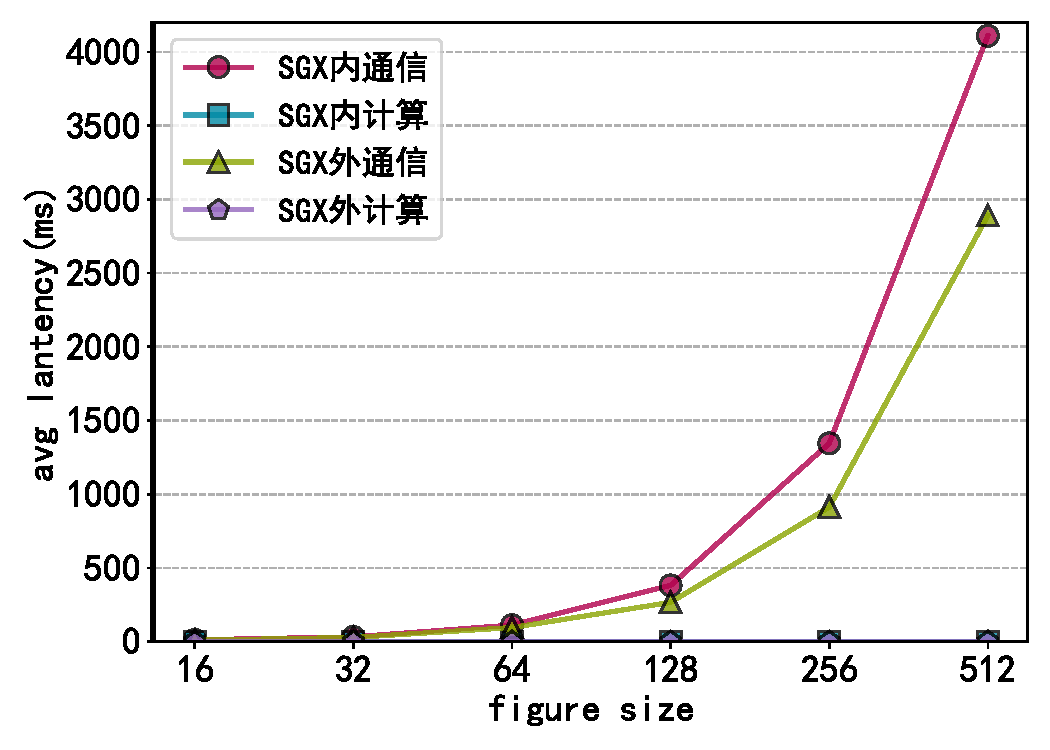
\includegraphics[width=.6\textwidth]{figures/evaluation.pdf}
    \caption{SGX内外微服务通信和计算耗时}
    \label{fig:evaluation}
\end{figure}

\subsection{安全分析}

如~\cref{subsec:threat-model}讲述的威胁模型所示,本次研究主要针对的攻击手段包括系统特权态攻击、网络攻击、漏洞利用攻击等攻击手段,重点防御隐私泄露问题,结合信任模型,我们可以得到如下的安全性分析:

\begin{itemize}
    \item \textbf{系统特权态攻击}:因为硬件和SGX是可信的,因此根据SGX的防御模型,即使OS或HyperVisor是恶意的或被劫持,SGX中的数据也不会泄露,因此本平台可以防御系统特权态攻击。
    \item \textbf{中间人攻击}:对于中间人攻击,我们使用了DHKE协议来协商对称共享密钥,用以加密保证通信的安全性;即使所有的DH共享参数都被中间人截获,中间人也无法得到密钥,因此无法解读加密信息。同时通过使用SGX远程验证,可以验证微服务节点身份的真实性,防止中间人伪造节点进行攻击。
    \item \textbf{重放攻击}:对于重放攻击,我们在通信协议中加入了计数器,且借助SGX和微服务计算场景的特点,消除了TLS 0-RTT状态恢复情况的漏洞,可以成功过滤掉重放攻击。
    \item \textbf{编程漏洞带来的攻击}:对于系统编程语言容易出现的悬垂指针、缓冲区溢出等漏洞带来的攻击,我们选择使用安全编程语言Rust,结合其强大的静态分析能力,基本可以消除这些情况(除非使用unsafe)。
    \item \textbf{权限扩散}:我们使用JWT的方法进行授权管理,类似于基于功能(Capability)的思想,为了防止权限扩散到下级节点,我们使用了Token交换的授权管理方法,可以实现细粒度的授权管理,减少隐私扩散。
\end{itemize}

另外,在一个完善的微服务场景中,还可能存在物理攻击、DDoS攻击、针对数据库的攻击等,但是针对这些攻击的应对措施与本次研究是正交的领域,因此不在本次研究的讨论范围内。

\clearpage
\section{讨\ 论}\label{sec:discussion}

\subsection{相关工作}

MSL da Silva等人~\cite{da2019squad}提出了Squad,通过一个SGX保护的数据存储节点,存储各个服务节点需要访问和使用的敏感数据,例如密钥、证书、配置信息等,同时可以对其他微服务进行验证,由此实现对微服务应用的保护。但是Squad节点可能会成为整个系统的性能和安全瓶颈。Squad与本文的设计并不是冲突的,Squad主要针对的是微服务应用启动和配置的问题,而本文主要为微服务提供了安全的运行时环境和安全高效的通信协议,保障了微服务运行时安全,因此可以配合使用共同致力于保护微服务的安全。

S Brenner等人~\cite{brenner2017secure}提出了Vert.x Vault,通过改进Eclipse Vert.x框架,使其能够同时支持使用C/C++语言编写的安全微服务节点和使用Java语言编写的普通节点,从而实现了借助SGX保护微服务的目的。但是Vert.x Vault的实现受限于特定框架和语言,且SGX中的程序仍需要使用C/C++语言重新编写,损失了灵活性且代价较高,而且不能防止编程漏洞引入的攻击,因此安全性和适用性都不如本文的设计。

对于SGX中的运行时,成熟的库操作系统包括Graphene-SGX~\cite{tsai2017graphene}、Occlum~\cite{shen2020occlum}等,而针对语言的运行环境包括Rust-SGX~\cite{wang2019towards}、GoTEE~\cite{ghosn2019secured}、Uranus~\cite{jiang2020uranus}、ScriptShield~\cite{wang2019running}等,分别尝试在飞地中运行Rust、Go、Java和脚本语言等。这些运行时的设计各有特点,本文的设计也参考了其中的多种设计;但是这些设计本身不一定适用于微服务的安全计算场景(例如引入额外的TCB),因此本文的运行时设计仍然有其独特的价值。

\subsection{未来展望}

对于基于可信执行环境的安全计算微服务场景,本文的工作仍有一些局限性,因此我们认为未来的工作可以从以下几个方面进行:

\begin{itemize}
    \item \textbf{通过进一步的分析解决隐私扩散问题。}尽管本文中使用了基于Token交换的细粒度授权管理方案,引入了额外的开销,但是仍然不能完全解决隐私扩散问题,例如微服务节点B将节点A的数据泄露给C,但是A并不希望C能够获取这些数据(受限于不同开发组之间的隐私协定),这一点无法使用Token授权完全避免。我们认为这是因为微服务节点间不能感知彼此的行为,即A不能得知和约束B对其发送过去的数据的处理方式,B将数据传递给C这件事A不知情也无法阻止。目前可以采用非技术的约束手段来减小这一问题,但是这样容易出现疏漏,因此我们需要进行进一步的研究,通过技术手段解决隐私扩散问题。
    \item \textbf{通过节点调度降低通信延迟。}微服务应用可以通过节点调度来降低通信延迟,例如将频繁通信的节点部署在同一个物理机上、同一个飞地中甚至是同一地址空间,这样可以大大减少通信延迟。但是这一点需要进一步的研究,达到在不降低安全性的前提下进行调度。
    \item \textbf{适配更多架构。}由于微服务应用具有异构性的特点,为了增强平台的适用性,需要进一步研究如何在不同的架构上实现本文的设计,达到类似的安全保障。
\end{itemize}

\clearpage
\section{总\ 结}\label{sec:conclusion}

我们设计并实现了一个基于可信执行环境的安全高效微服务计算平台,包含一个细粒度、模块化的运行时系统以及一个安全高效的通信协议。该平台针对微服务安全计算场景的特点,能够保障运行环境的安全性和通信的安全和高效性。我们的运行时具有较小的TCB,并通过借助Intel SGX提供的保护,可以避免特权态攻击;我们的安全通信协议结合了TLS和SGX远程验证的特点,能够防御中间人攻击和重放攻击,确保通信节点的合法性,并能够实现更小的通信延迟。我们在该平台上实现了一个简单的图像处理微服务示例应用,并对其进行了测试。测试结果表明,该平台在安全性和性能上都能满足微服务安全计算场景的需求。

\clearpage


\nocite{*} % 将所有的参考文献都加入到列表中
\addcontentsline{toc}{section}{参考文献}
\bibliography{note}

\clearpage
\section*{谢\ 辞}
\addcontentsline{toc}{section}{谢辞}

在本次毕业设计过程中乃至整个大学生涯中,我得到了太多太多的鼓励和帮助,以至于不知从何说起。以下感谢信息随感而发,不分先后。

感谢我的本科生导师沈坚老师,是您耐心的指导引领我步入了计算机的世界。

感谢香港大学崔鹤鸣老师对我的赏识,未来我将在您的指导下开启下一段研究生涯。

感谢邓蓉老师,激发了我对计算机系统的兴趣,并为我的毕业设计提供了帮助和指导。

感谢叶晨老师,为我本科阶段的专业竞赛提供大力帮助和支持。

感谢赵君峤老师,您的每一门课都让我受益匪浅。

感谢辅导员刘谦老师和刘梦露老师,您们的工作让我的生活和学业少了很多烦恼。

感谢班主任王力生老师,悉心帮我解决生活上的困难。

感谢叶茂尧、李博宇、李嘉庚、范正源、张琦竣等学长,为我提供了许多帮助和经验,对我的本科生涯产生了不可磨灭的影响。

感谢一路走来的舍友高志成、尚丙奇、张淞皓、戴浏、王上游、白瑾辰、董浩同学,与你们的友好相处让我的大学生活从不孤单。

感谢我的算法竞赛队友张馨月、钟伊凡,与你们一起训练和比赛让我感受到了团队的力量。

感谢我的好朋友武澳奇和游康,我从你们身上学到了很多,和你们相处的时光最为轻松惬意。

感谢和我比较熟悉的汪冰海、范千惠、刘孔阳、孔庆晨、许辰昊、刘云帆、刘羽茜、马家昱、彭瀚等同学,很荣幸能够认识你们,和你们的友谊为我的大学生活增添了很多美好的回忆。

感谢香港大学的Jianyu、Siyuan、Huangdong、Shixiong、Frank、Tianxiang、Zekai等师兄,感谢你们引导我踏入科研的大门,并帮助我更快地熟悉香港的生活。

感谢上海实验室实习期间认识的的林坤、布清文、苗成林等同学和同事,和你们的交流让我的实习生活不再枯燥。

感谢罗格峰同学,与你在一起的时光是我大学中最美好的回忆。

感谢我的父母,感谢你们一路以来为我的付出和支持,感谢你们在我人生坎坷时无私的帮助,感谢你们对我每一个决定的尊重,我爱你们。

感谢对我施以善意的的每一个人,感谢那个青春无悔的自己。


\end{document}
